\newpage
\begin{figure}[h!]
    \centering
    \caption{Timeline for university application in the UK}
    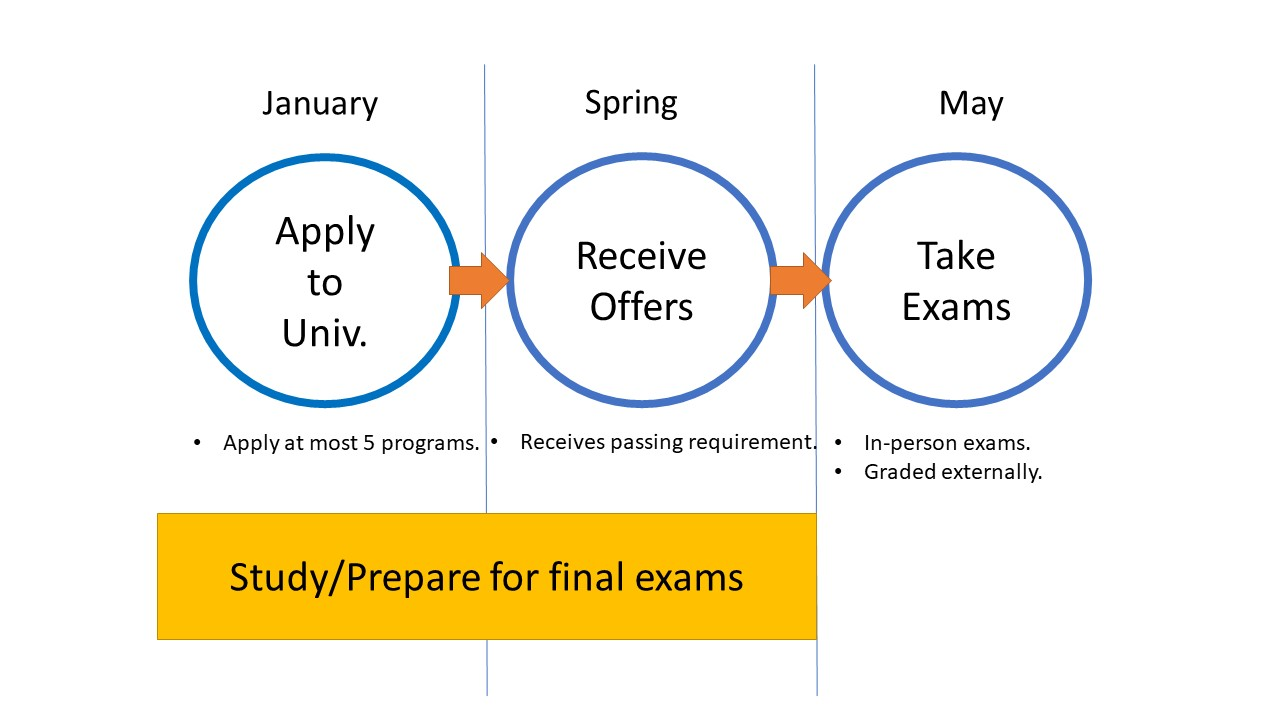
\includegraphics[width=\linewidth]{figures/Background/Timeline_Shrink.jpg}
    \label{fig:enter-label}
\end{figure}
\clearpage

\begin{figure}[!htbp]
    \centering
    \caption{Cohort Size Growth}
    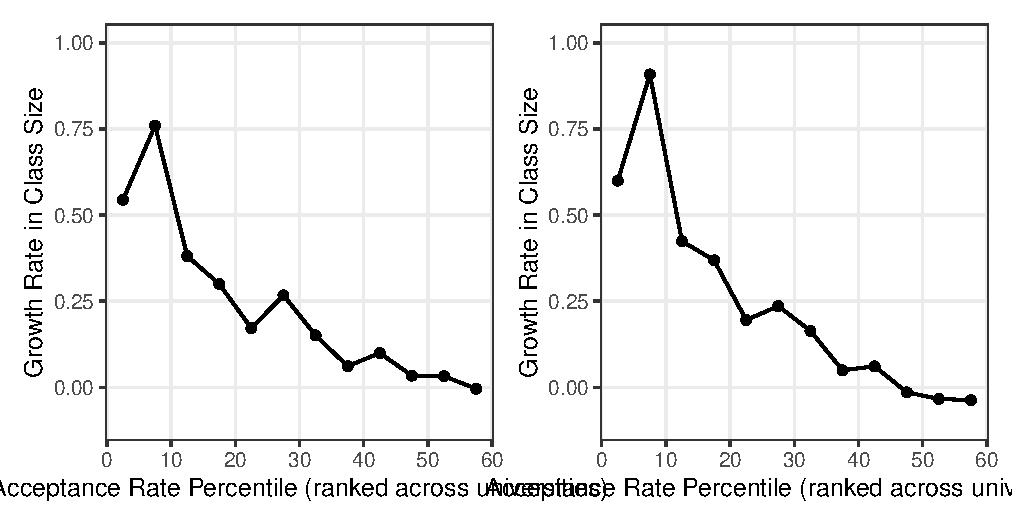
\includegraphics[width=\linewidth]{figures/Background/Growth_Rate_Acceptance_through_Any.pdf}
    \label{fig:CohortSizeGrowthAny}

  \vspace{4pt} % small gap between panels

  \begin{subfigure}[t]{\linewidth}
    \centering
    \caption{Cohort Size Firm Growth}
    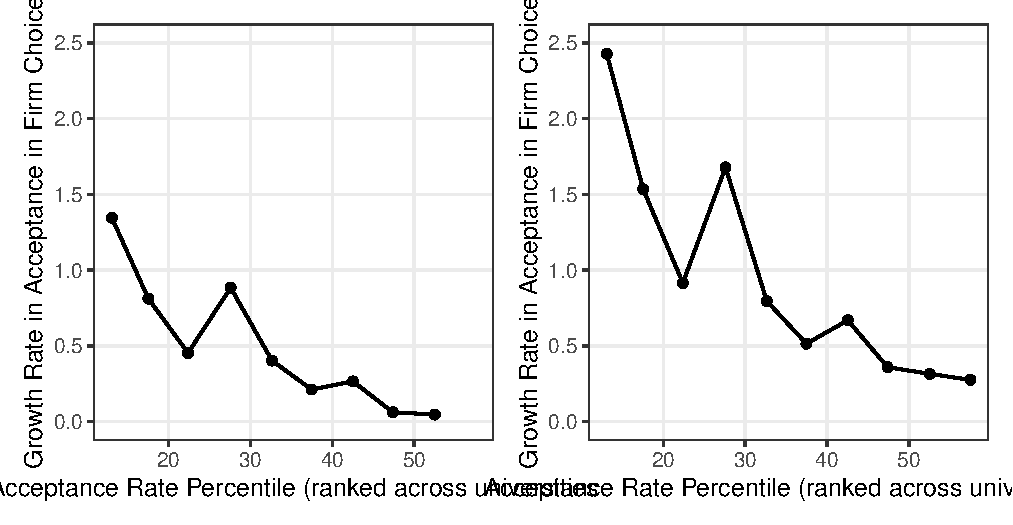
\includegraphics[width=\linewidth]{figures/Background/Growth_Rate_Acceptance_through_Firm.pdf}
    \label{fig:CohortSizeGrowthFirm}
  \end{subfigure}
  \label{fig:inflation_subjects_20_21}
\end{figure}
\clearpage

\begin{figure}[!h]
    \centering
    \caption{Grade inflation by school quality (2020, 2021).}
    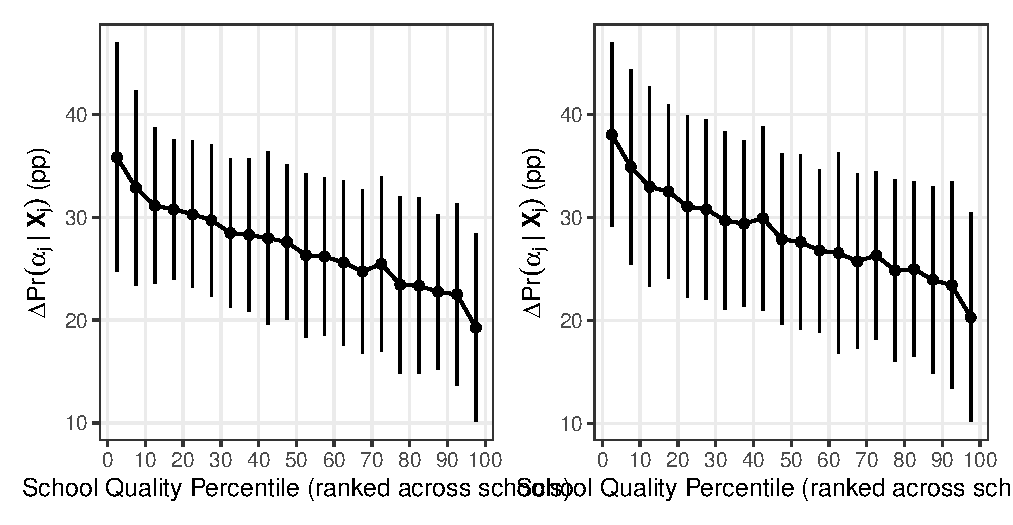
\includegraphics[width=\linewidth]{figures/Results/treatment_effects_by_schoolquality.pdf}
    \label{fig:inflation_main}
\end{figure}
\clearpage

\begin{figure}
    \centering
    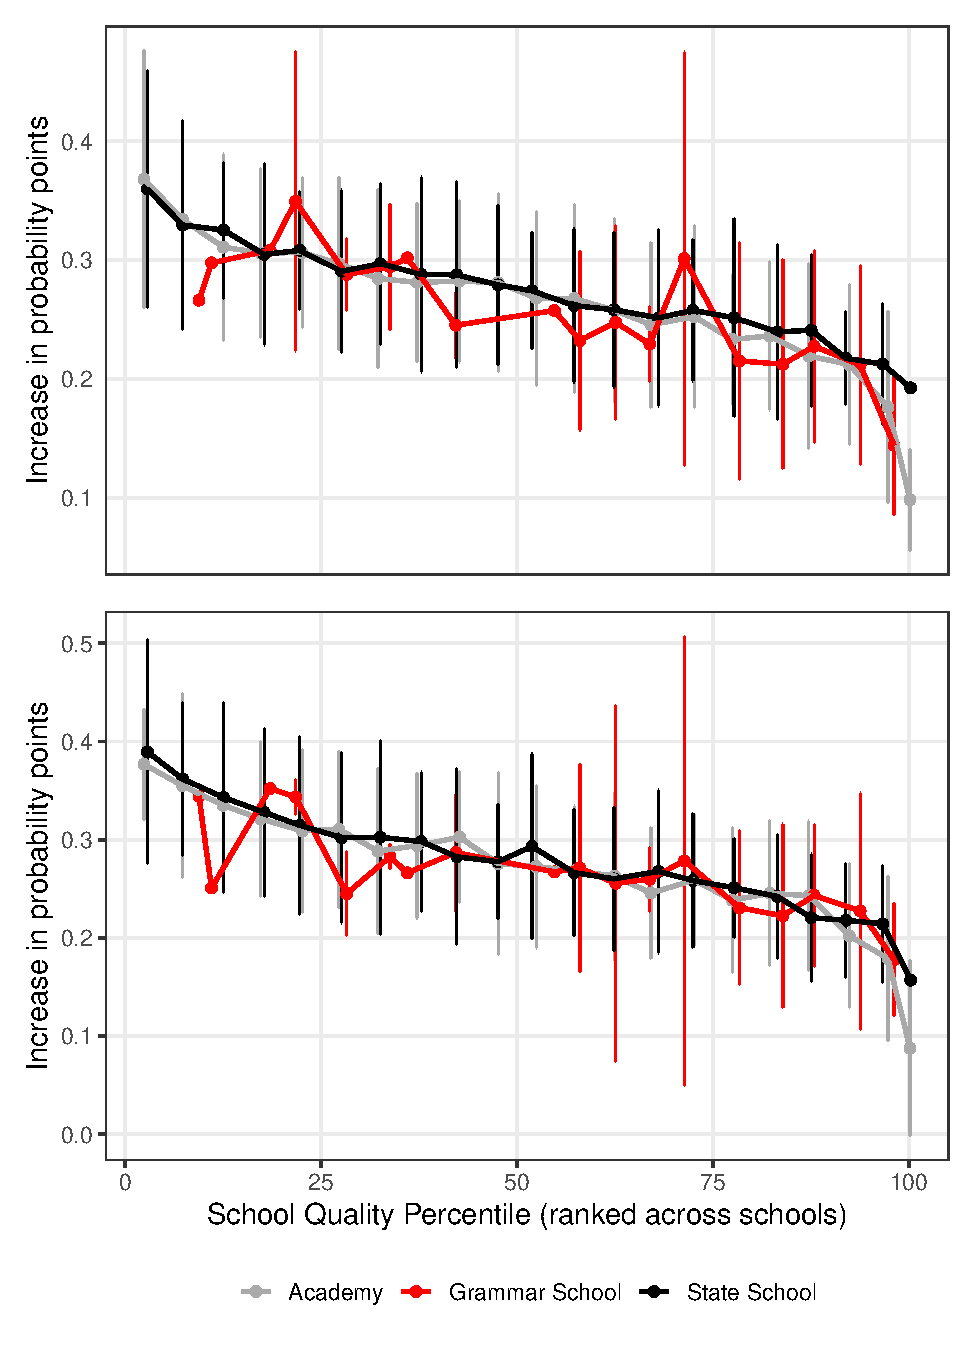
\includegraphics[width=\linewidth]{figures/Appendix/treatment_by_schooltype_grammar.pdf}
    \caption{Grade inflation at grammar schools}
    \label{fig:treatment_type_grammar}
\end{figure}

\begin{figure}
    \centering
    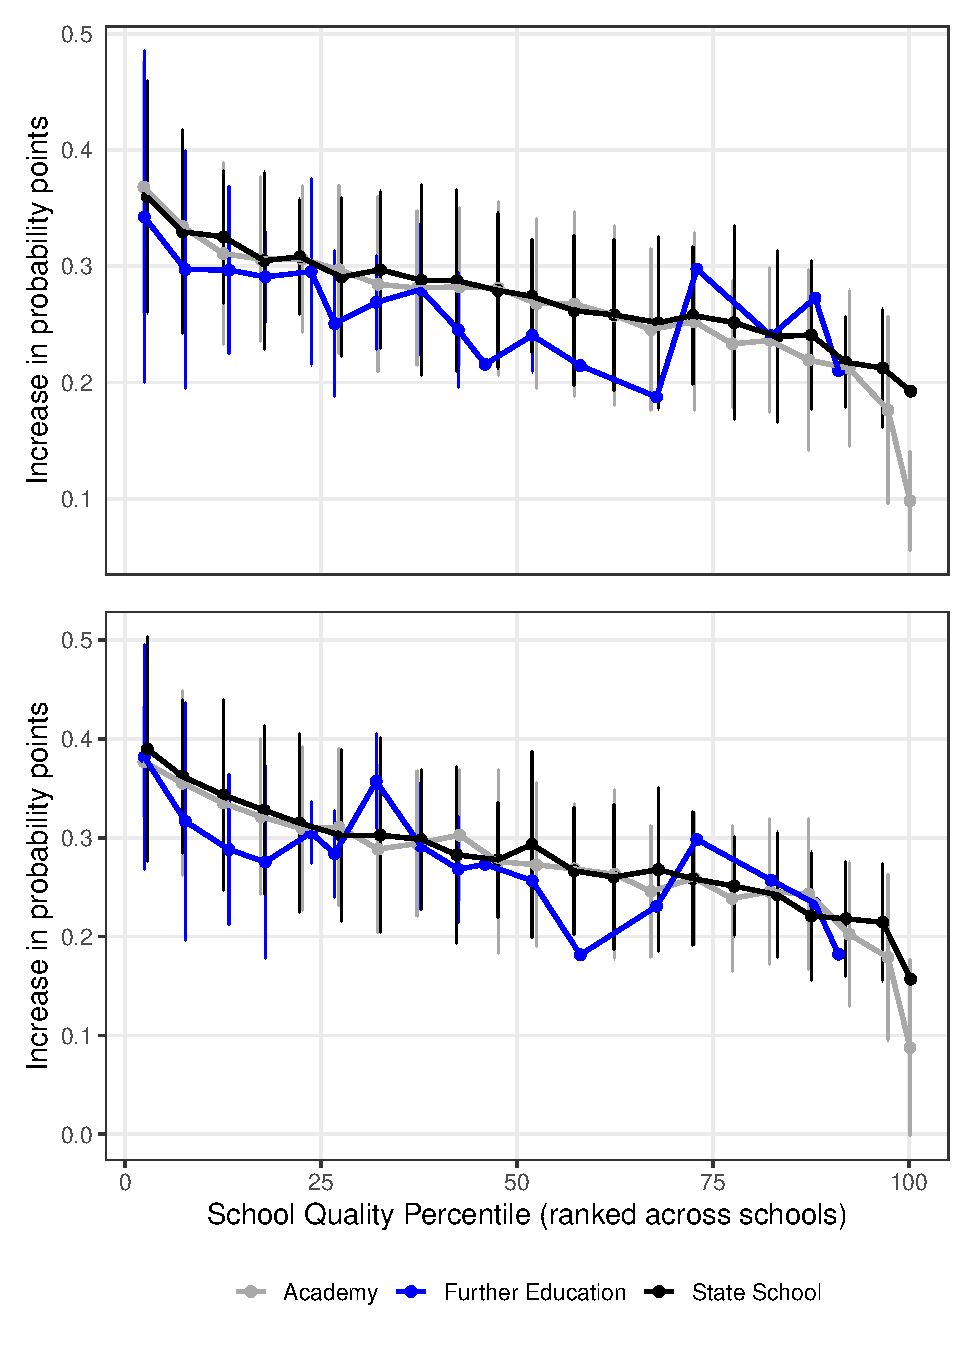
\includegraphics[width=\linewidth]{figures/Appendix/treatment_by_schooltype_further.pdf}
    \caption{Grade inflation at further education schools}
    \label{fig:treatment_type_further}
\end{figure}

\begin{figure}[!htbp]
    \centering
    \caption{Relative risk reduction by school quality percentile, by school type (true vs pooled vs separate)}
    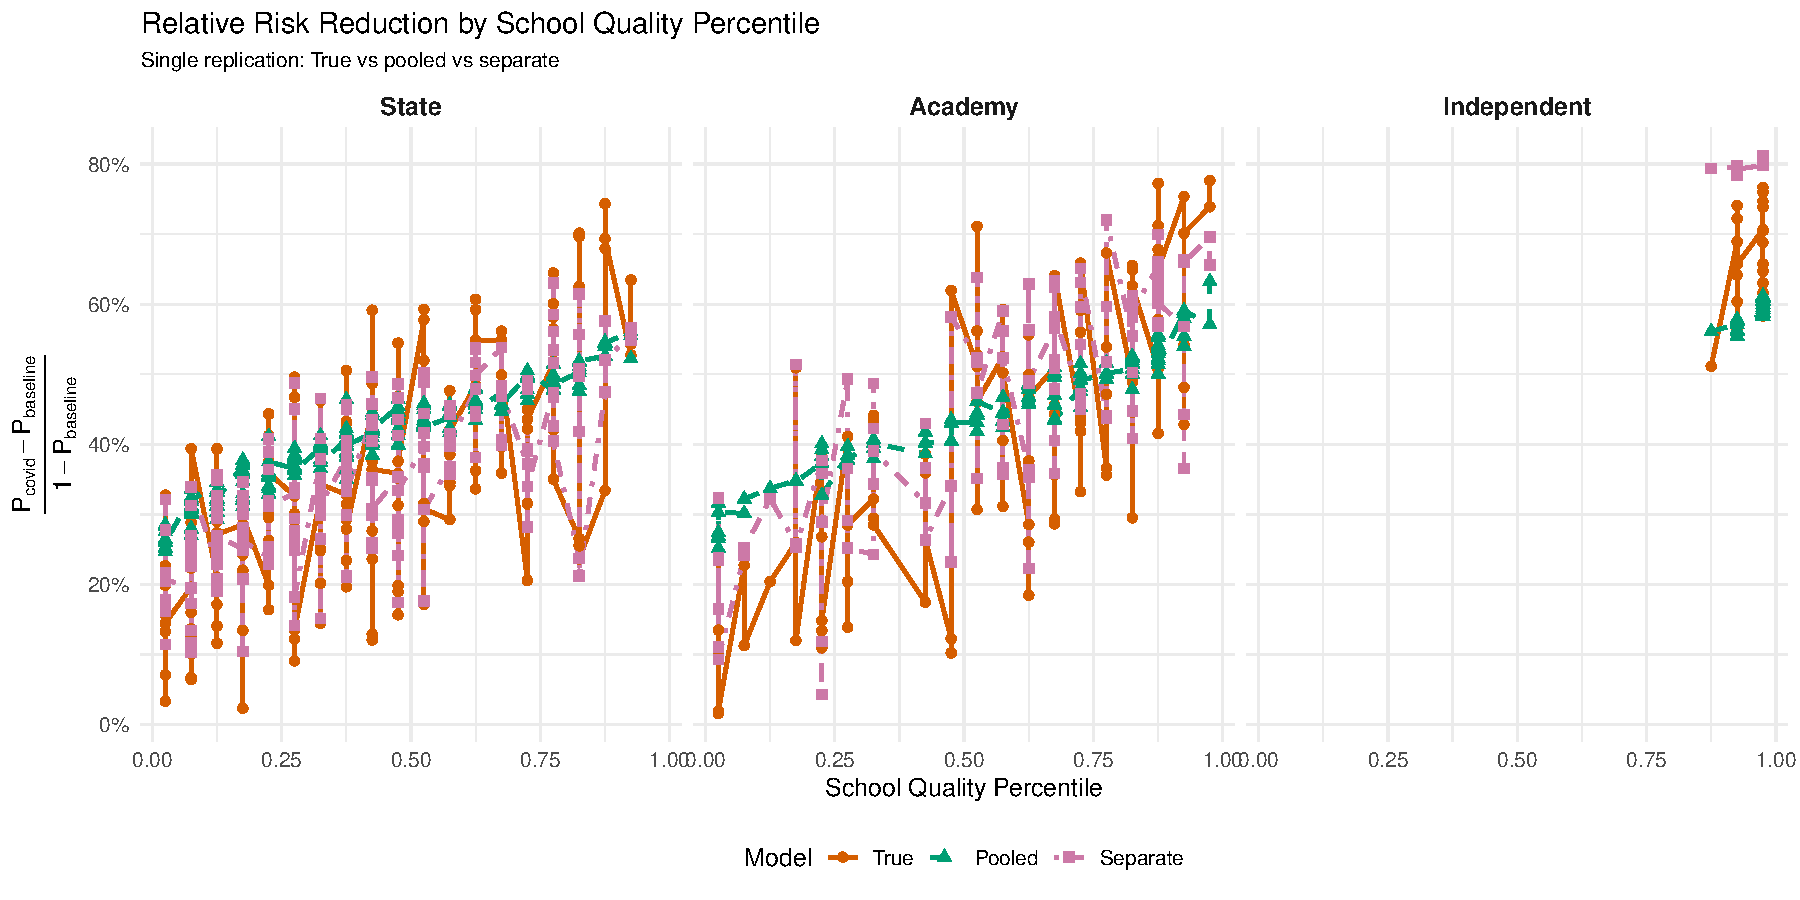
\includegraphics[width=\linewidth]{figures/Appendix/rrr_schooltype_sim.pdf}
    \label{fig:rrr_schooltype_sim}
\end{figure}

\begin{figure}[!htbp]
  \centering
  \caption{Grade inflation by GCSE score by exam subject.}
  \begin{subfigure}[t]{\linewidth}
    \centering
    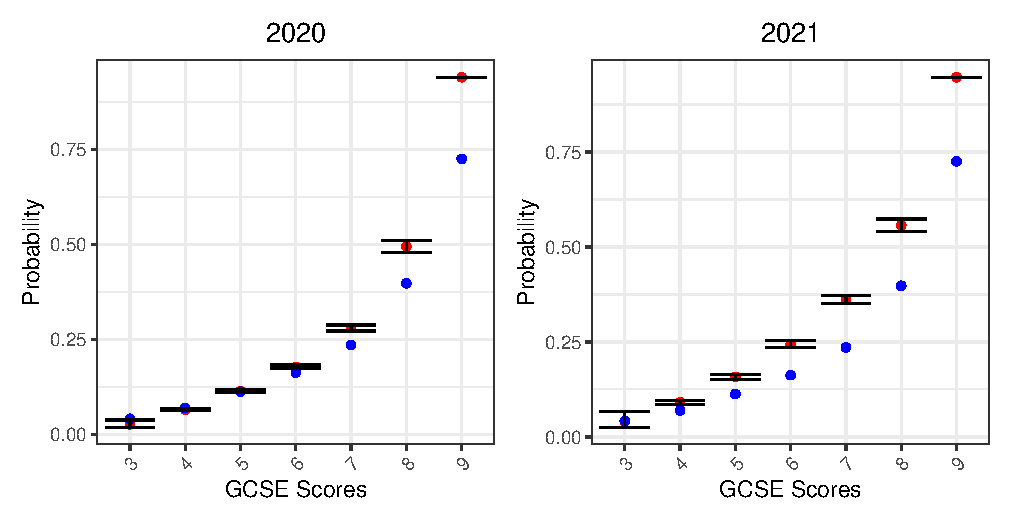
\includegraphics[width=0.94\linewidth]{figures/Results/ByGCSE_bins.pdf}
    \caption{Grade inflation by GCSE score in Mathematics}
    \label{fig:gcse_math}
  \end{subfigure}

  \vspace{0.8em}

  \begin{subfigure}[t]{\linewidth}
    \centering
    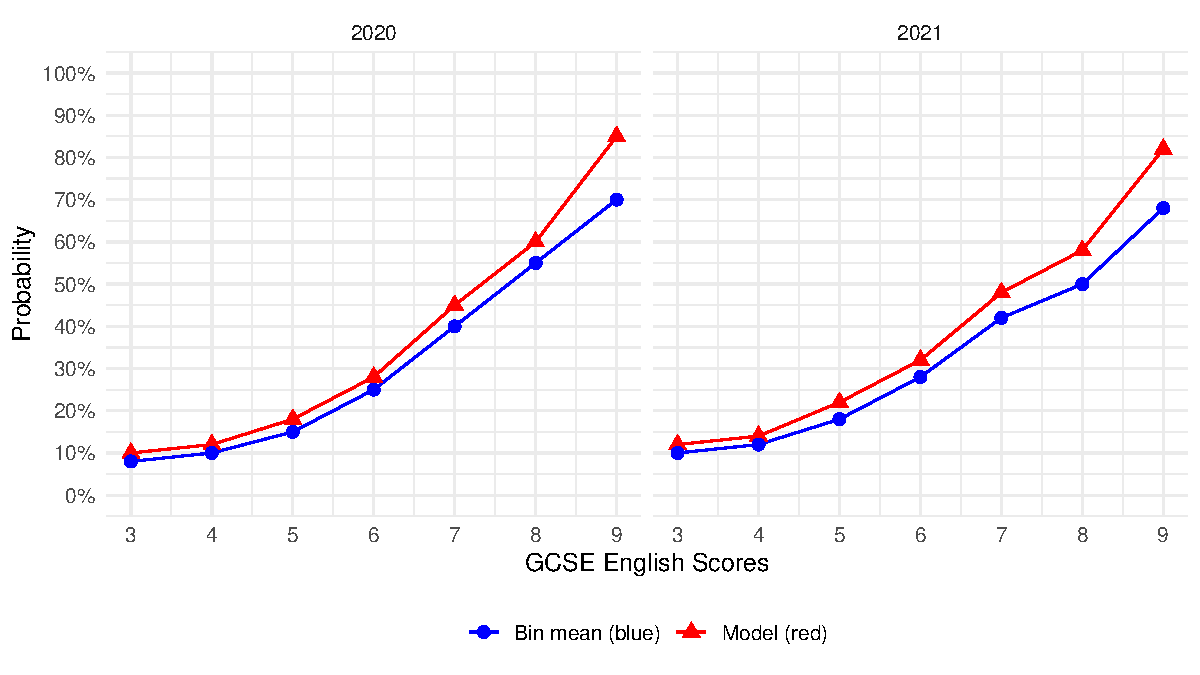
\includegraphics[width=0.94\linewidth]{figures/Results/gcse_eng_prob_panels.pdf}
    \caption{Grade inflation by GCSE score in English Literature.}
    \label{fig:gcse_eng}
  \end{subfigure}

  \label{fig:gcse_combined}
\end{figure}

\begin{figure}[!h]
    \centering
    \caption{Inflation by parental occupation class}
    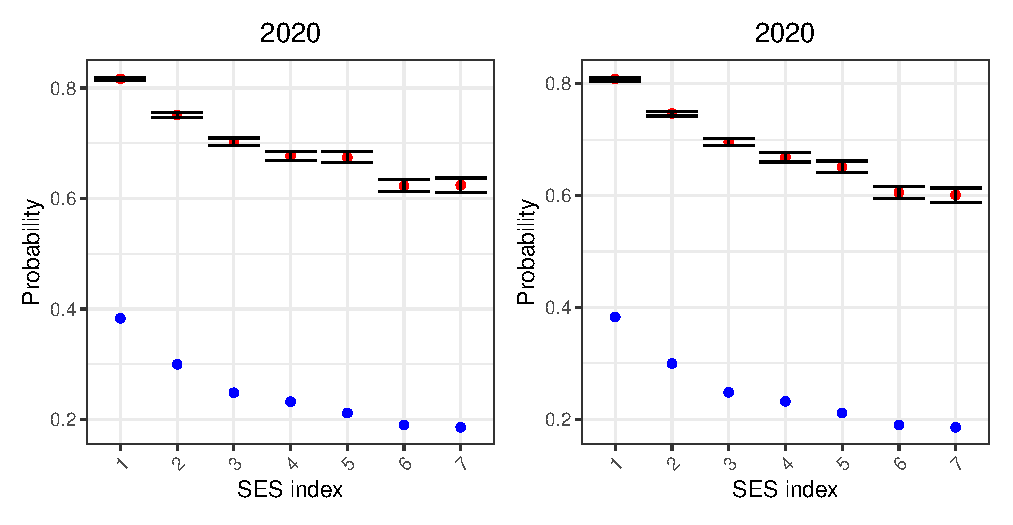
\includegraphics[width = \linewidth]{figures/Results/BySES_bins.pdf}
    \label{fig:ses_agg}
\end{figure}


\begin{figure}[!htbp]
  \centering
  \caption{Grade inflation by (a) Parental occupation class, and (b) Univ. progression rate}
  \begin{subfigure}[t]{\linewidth}
    \centering
    \caption{}
    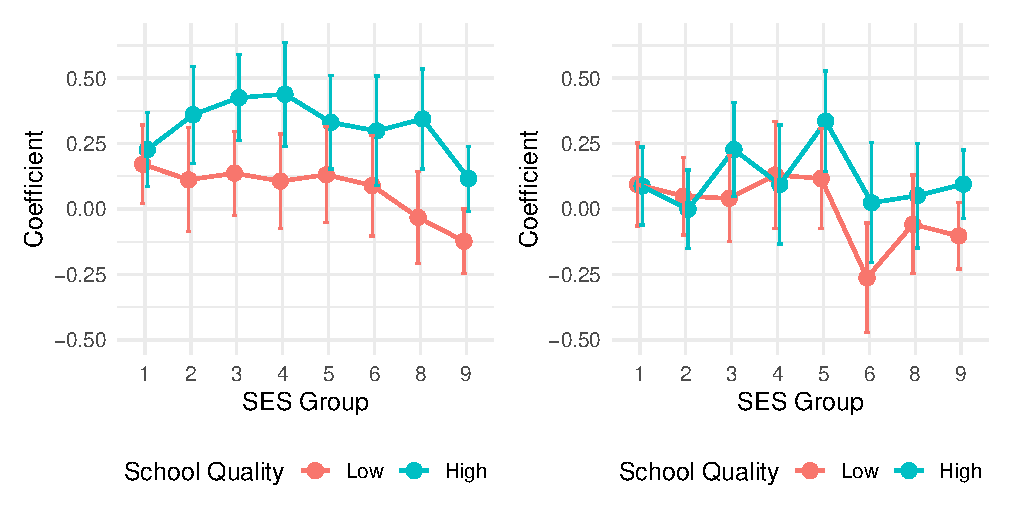
\includegraphics[width = \linewidth]{figures/Results/SES_BySchoolQuality_A.pdf}
    \label{fig:SES_bySQ}
  \end{subfigure}

  \vspace{0.8em}

  \begin{subfigure}[t]{\linewidth}
    \centering
    \caption{}
    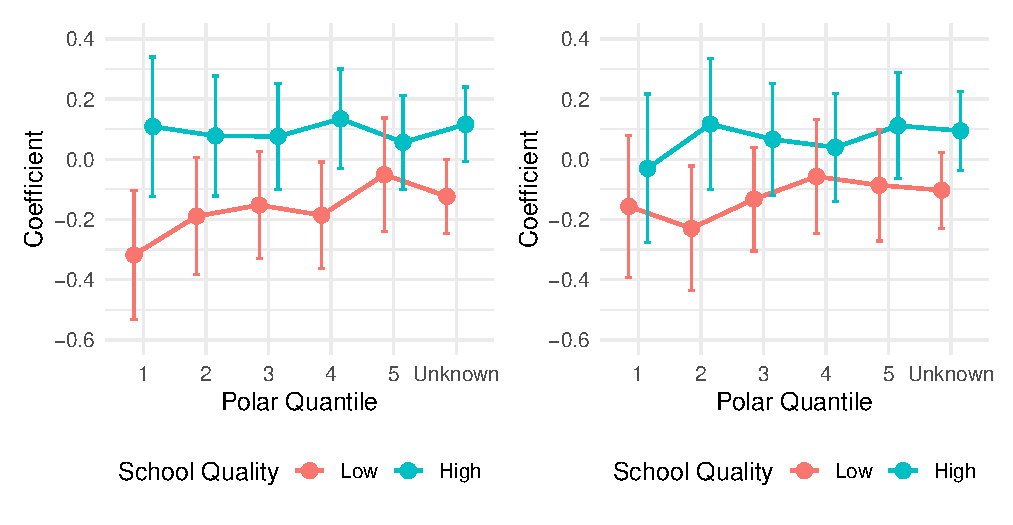
\includegraphics[width = \linewidth]{figures/Results/POLAR_BySchoolQuality_A.pdf}
    \label{fig:SES_bySQ}
  \end{subfigure}

  \label{fig:income_SQ_combined}
  \caption*{\footnotesize Note: The bin-scatter displays student level difference in grade improvements across (a) parental occupational class and (b) average university progression rate of the students' residential address. The sample is the universe of A-level exams used for admissions at British universities through the centralized administrative system (N = 2,802,651). Year-specific coefficients and 95\% confidence intervals are from a logistic regression that regresses a success dummy indicating the student receiving a top grade (A or $\text{A}^*$) on the interaction between school subject group dummy and a time indicator for both pandemic years. The regression controls for students' achievement score in a previous standardized national exam (GCSE) in mandatory subjects (mathematics and English literature) and a dummy variable for the subject course of the exam. Standard errors are clustered at the school-subject course level. }
\end{figure}
\clearpage



\begin{figure}[!h]
    \centering
    \caption{Inflation by poverty score score}
    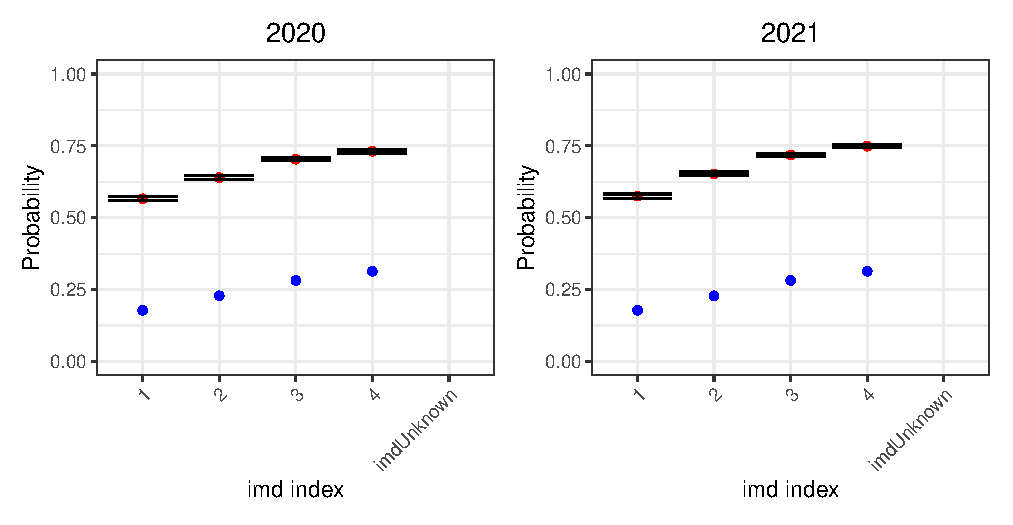
\includegraphics[width = \linewidth]{figures/Results/ByIMD_bins.pdf}
    \label{fig:imd_agg}
\end{figure}
\clearpage


\begin{figure}
    \centering
    \caption{Inflation by GCSE scores measured by log-odds}
    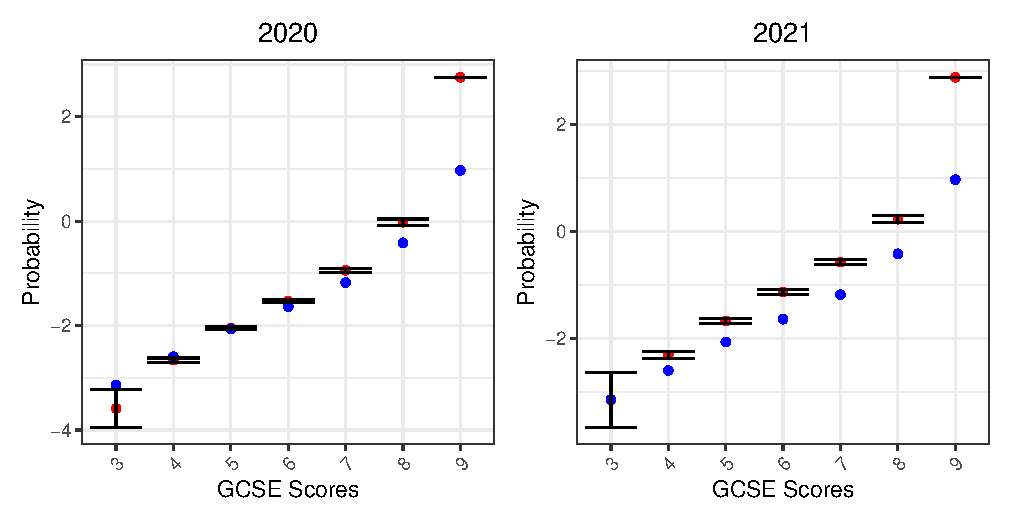
\includegraphics[width=\linewidth]{figures/Results/ByGCSE_bins_logit.pdf}    
    \label{fig:GCSE_math_logit}
\end{figure}
\clearpage

\begin{figure}
    \centering
    \caption{Inflation by GCSE scores by school quality}
    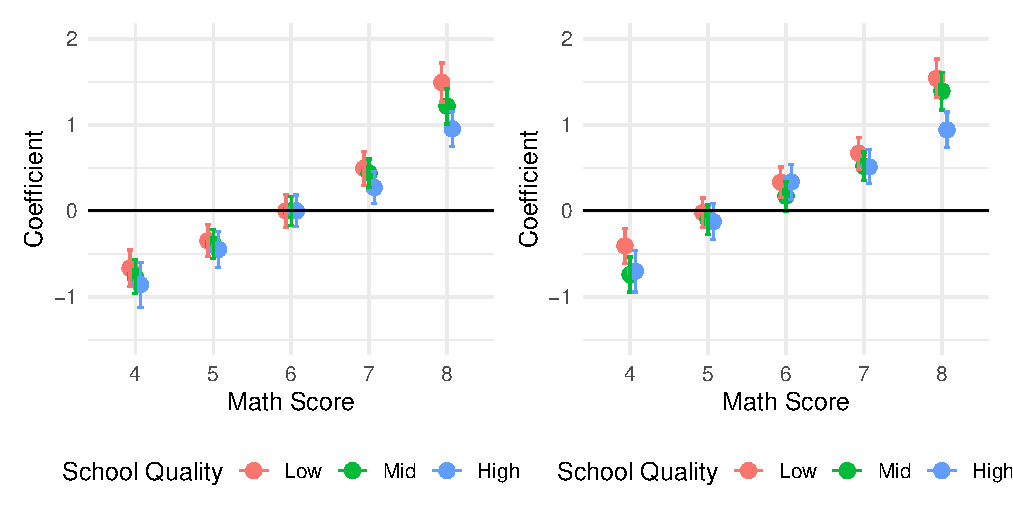
\includegraphics[width=\linewidth]{figures/Results/MathGCSE_BySchoolQuality_A_20+21.pdf}
    
    \label{fig:gcse_bySQ}
\end{figure}
\clearpage

\begin{figure}[!h]
    \centering
    \caption{Inflation by GCSE scores and schools}
    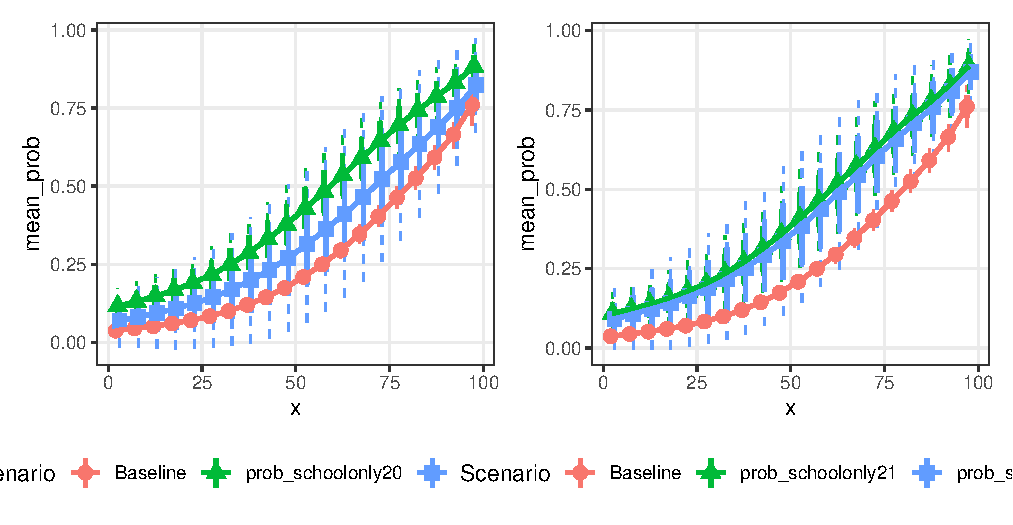
\includegraphics[width = \linewidth]{figures/Results/SchoolAndGCSE.pdf}
    \label{fig:gcse_vs_school}
\end{figure}
\clearpage

\begin{figure}
    \centering
    \caption{Effect of inflation on placements in 2020}
    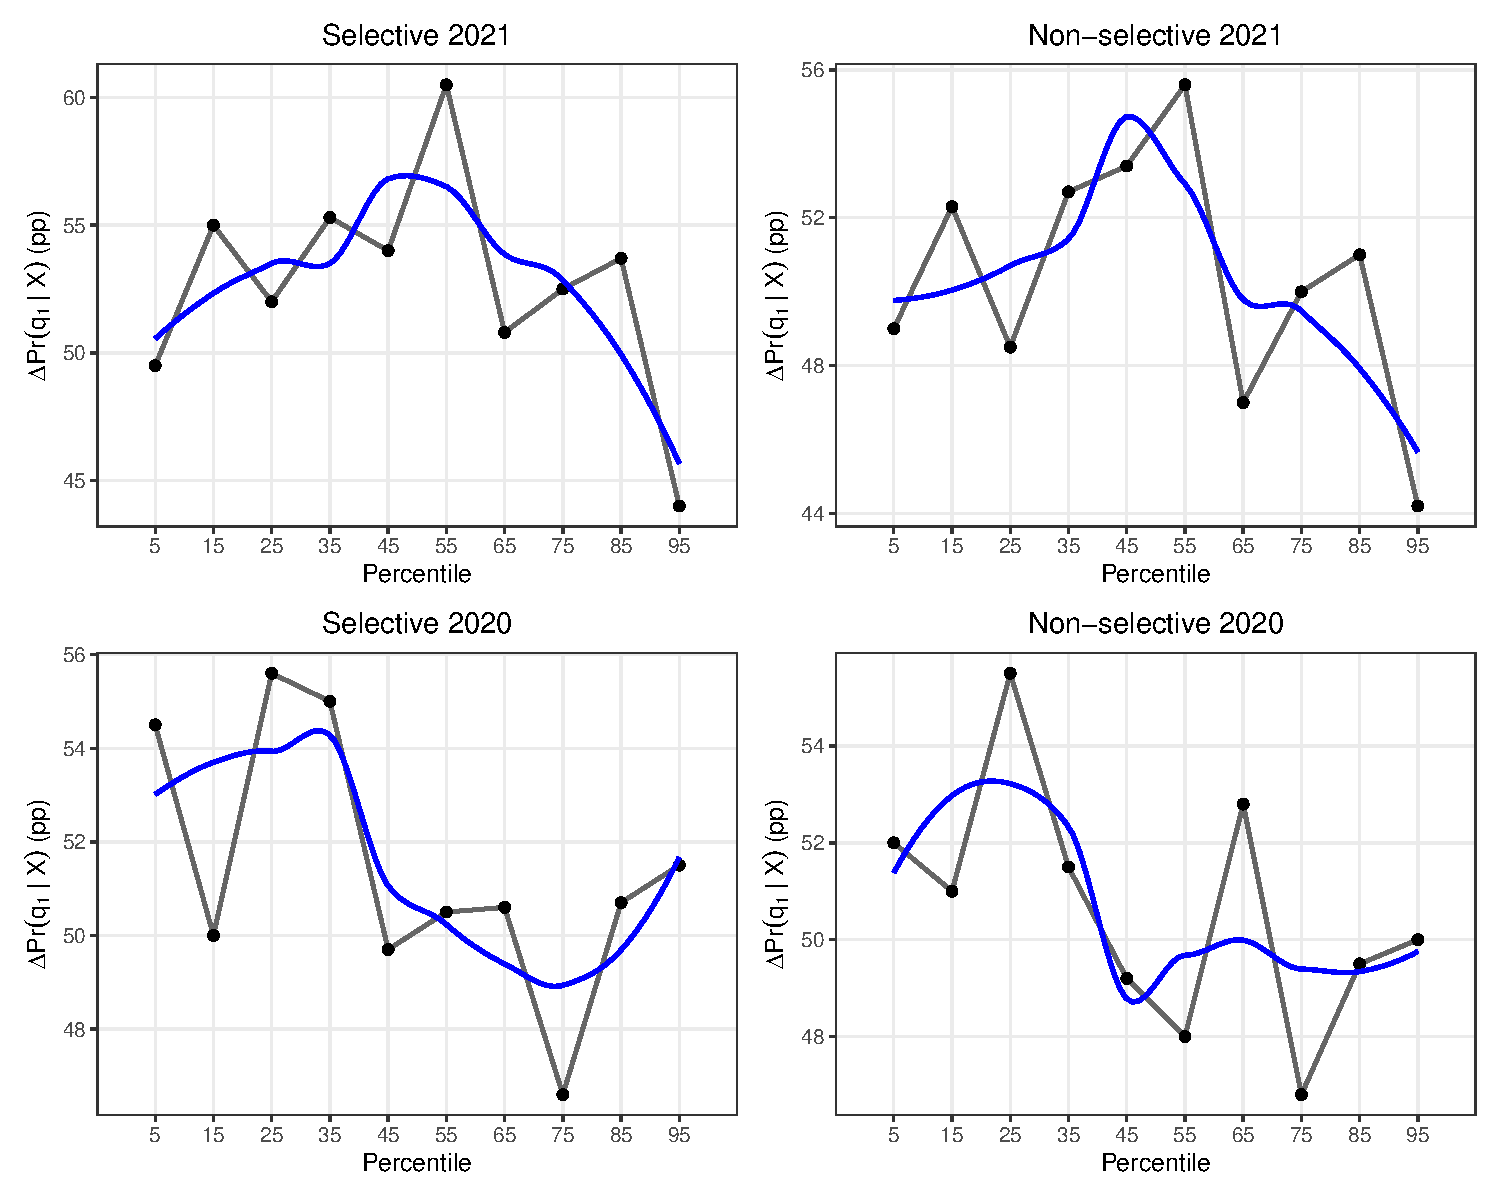
\includegraphics[width=\linewidth]{figures/Results/plots_selective_nonsel.pdf}
    \label{fig:placement_sel}
\end{figure}

\begin{figure}
    \centering
    \caption{Effect of inflation on placements in 2021}
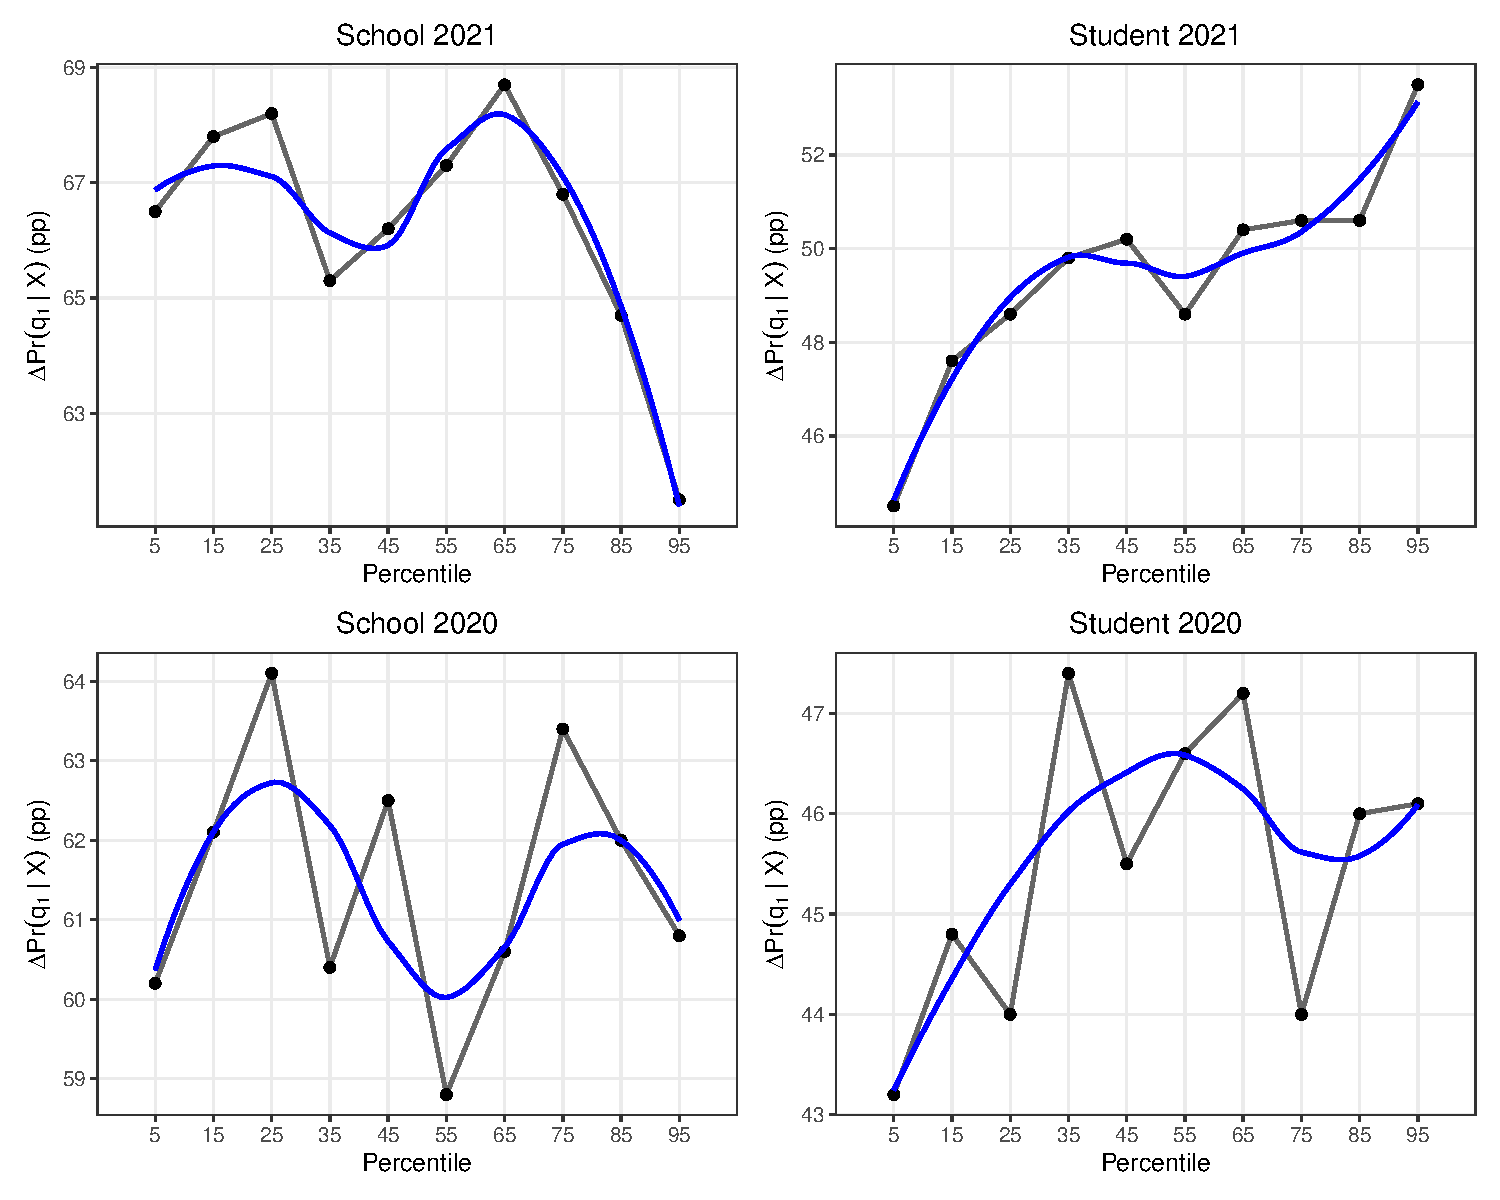
\includegraphics[width=\linewidth]{figures/Results/plots_school_student.pdf}
    \label{fig:placement_channel}
\end{figure}
\clearpage

\begin{figure}[!htbp]
  \caption{Impact of grade inflation into placement success rates by school. }
  \centering
  \begin{subfigure}[t]{\linewidth}
    \centering
    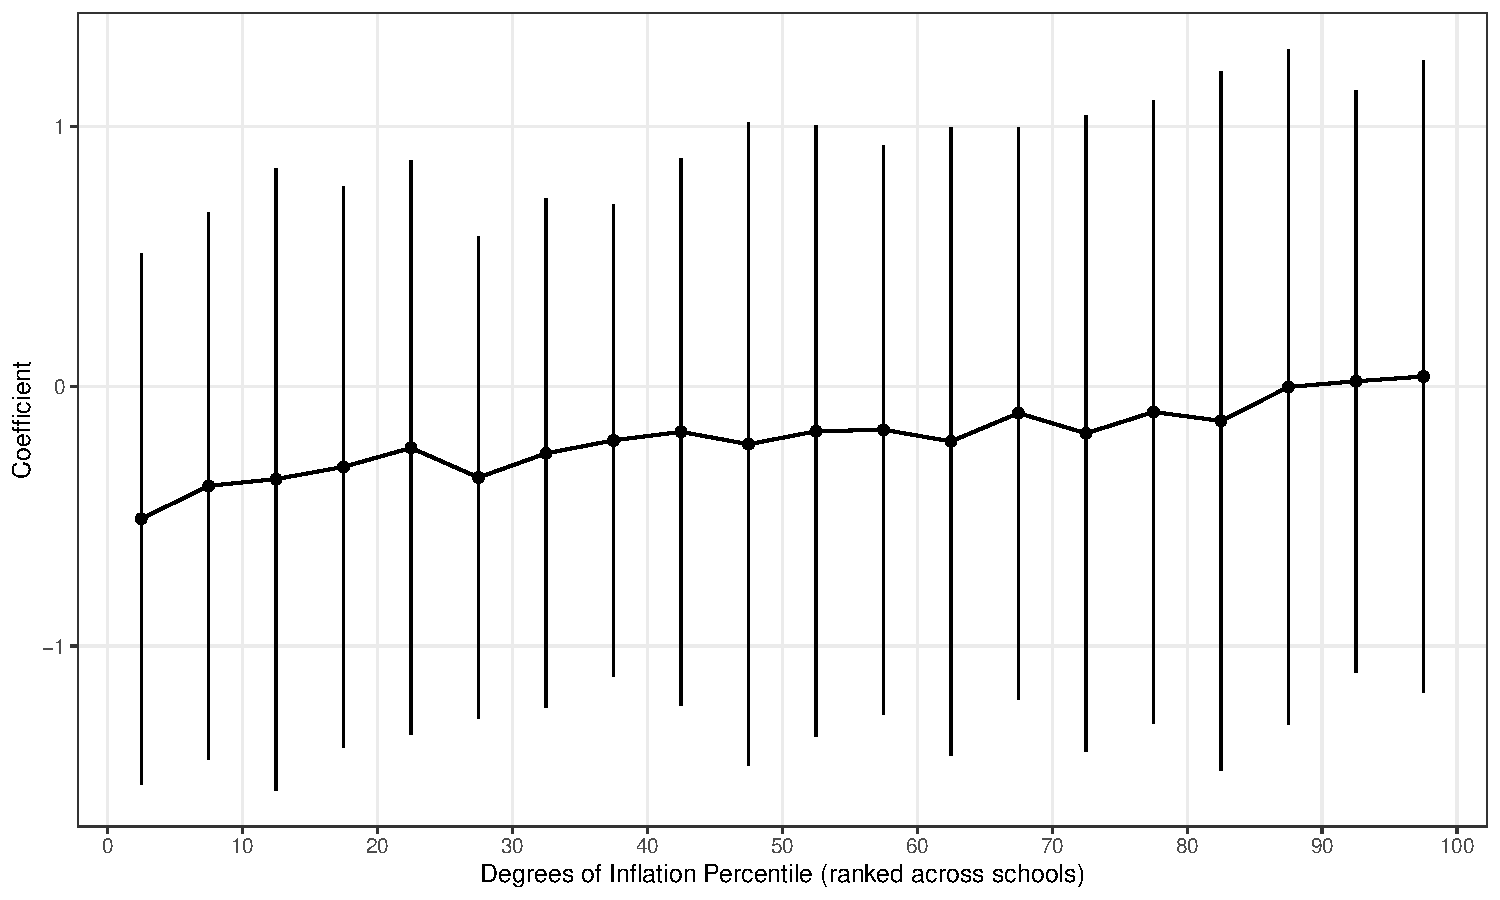
\includegraphics[width=\linewidth]{figures/Results/Placement_Success_A.pdf}
    \caption{Grade inflation by subject group, 2020.}
    \label{fig:inflation_subject20}
  \end{subfigure}

  \vspace{4pt} % small gap between panels

  \begin{subfigure}[t]{\linewidth}
    \centering
    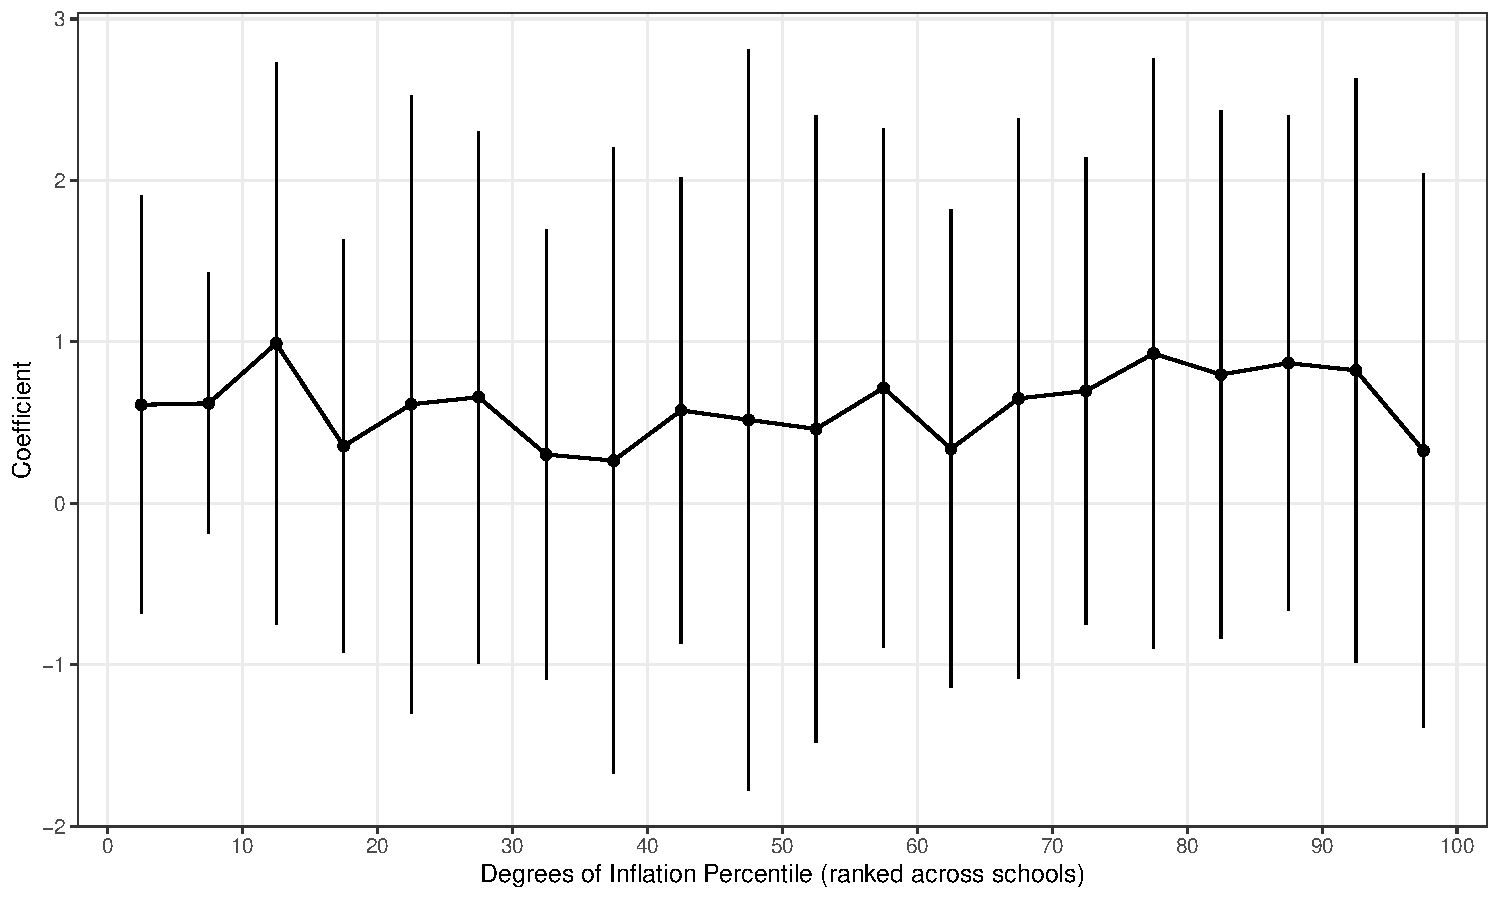
\includegraphics[width=\linewidth]{figures/Results/Placement_Selective_A.pdf}
    \caption{Grade inflation by subject group, 2021.}
    \label{fig:inflation_subject21}
  \end{subfigure}
  \label{fig:inflation_subjects_20_21}
\end{figure}

\begin{table}[htbp]\centering
\caption{Balance Table of Applicant Characteristics}
\resizebox{\textwidth}{!}{%
\begin{tabular}{lcccc}
\toprule
Characteristic & $N=1,192,935$ (2020) & $N=219,929$ (2021) & $N=234,294$ (2020 + 2021) & $N=1,647,158$ (2015-2019) \\
\midrule
\textbf{Gender} \\
Men    & 522,795 (44\%) & 95,289 (43\%) & 102,174 (44\%) & 720,258 (44\%) \\
Women  & 670,140 (56\%) & 124,640 (57\%) & 132,120 (56\%) & 926,900 (56\%) \\
\midrule
\textbf{School Type} \\
Academy          & 411,969 (35\%) & 84,186 (38\%) & 90,521 (39\%) & 586,626 (36\%) \\
Further Education& 62,864 (5.3\%) & 9,840 (4.5\%) & 10,614 (4.5\%) & 83,318 (5.1\%) \\
Grammar School   & 55,818 (4.7\%) & 5,897 (2.7\%) & 6,252 (2.7\%) & 67,973 (4.1\%) \\
Independent      & 167,995 (14\%) & 24,869 (11\%) & 26,301 (11\%) & 223,561 (14\%) \\
Sixth Form       & 237,426 (20\%) & 46,177 (21\%) & 48,868 (21\%) & 332,471 (20\%) \\
State School     & 256,863 (22\%) & 48,960 (22\%) & 51,738 (22\%) & 344,140 (21\%) \\
\midrule
\textbf{Ethnic Group} \\
Asian            & 156,871 (13\%) & 29,111 (13\%) & 30,869 (13\%) & 235,067 (14\%) \\
Black            & 61,526 (5.2\%) & 11,964 (5.4\%) & 12,568 (5.4\%) & 86,058 (5.2\%) \\
Mixed            & 53,751 (4.5\%) & 11,936 (4.5\%) & 13,335 (5.7\%) & 79,022 (4.8\%) \\
Other            & 51,823 (4.3\%) & 8,774 (4.0\%) & 9,207 (3.9\%)  & 69,804 (4.2\%) \\
Unknown/Prefer NS& 41,923 (3.5\%) & 7,936 (3.6\%) & 7,817 (3.3\%)  & 57,676 (3.5\%) \\
White            & 857,238 (72\%) & 144,645 (66\%)& 152,763 (65\%)& 1,154,617 (70\%) \\
\midrule
\textbf{Domicile} \\
England          & 1,070,768 (90\%) & 210,220 (96\%) & 224,699 (96\%) & 1,505,687 (91\%) \\
EU (excl. UK)    & 36,002 (3.0\%) & 6173 (2.8\%) & 6456 (2.8\%) & 48,631 (3.0\%) \\
Northern Ireland & 46,319 (3.9\%) & 1764 (0.8\%) & 1698 (0.7\%) & 49,781 (3.0\%) \\
Not EU           & 30,252 (2.5\%) & 5,535 (2.5\%) & 5,283 (2.3\%) & 41,070 (2.5\%) \\
Scotland         & 2,503 (0.2\%)  & 1,477 (0.7\%) & 2,310 (1.0\%) & 3,928 (0.2\%) \\
Wales            & 39,491 (3.3\%) & 1352 (0.6\%) & 1588 (0.7\%) & 42,431 (2.6\%) \\
\midrule
\textbf{POLAR4 Quintile} \\
Q1 & 113,733 (9.5\%) & 21,763 (9.9\%) & 23,175 (9.9\%) & 158,671 (9.6\%) \\
Q2 & 163,860 (14\%) & 29,981 (14\%)  & 32,260 (14\%) & 226,101 (14\%) \\
Q3 & 211,895 (18\%) & 41,877 (17\%)  & 44,111 (19\%) & 291,461 (18\%) \\
Q4 & 268,260 (22\%) & 49,360 (22\%)  & 52,248 (22\%) & 369,868 (22\%) \\
Q5 & 400,492 (34\%) & 74,065 (34\%)  & 79,426 (34\%) & 553,918 (34\%) \\
Unknown & 34,758 (2.9\%) & 6345 (2.9\%) & 6036 (2.6\%) & 47,139 (2.9\%) \\
\midrule
\textbf{IMD Quintile} \\
Q1 & 151,778 (13\%) & 30,905 (14\%) & 32,784 (14\%) & 215,467 (13\%) \\
Q2 & 186,674 (16\%) & 36,096 (16\%) & 38,057 (16\%) & 260,827 (16\%) \\
Q3 & 220,488 (18\%) & 39,982 (18\%) & 42,878 (18\%) & 303,348 (18\%) \\
Q4 & 162,748 (22\%) & 46,752 (21\%) & 47,873 (20\%) & 310,122 (19\%) \\
Q5 & 336,024 (28\%) & 59,774 (27\%) & 64,598 (28\%) & 460,396 (28\%) \\
Unknown & 35,223 (3.0\%) & 6420 (2.9\%) & 6100 (2.6\%) & 47,743 (2.9\%) \\
\bottomrule
\end{tabular}
}
\label{tab:balance}
\end{table}

\clearpage

\begin{table}[h!]
\centering
\caption{Distribution by Social Class, School Background, and Ethnic Group across University Types}
\label{tab:university_distribution}
\begin{tabular}{lccc}
\hline
\textbf{Category}                   & \textbf{Russell Group} & \textbf{Other Old} & \textbf{New} \\ \hline
\textbf{Social class origin}        &                       &                   &              \\
Higher professional/managerial      & 35                    & 23                & 42           \\
Lower professional/managerial       & 25                    & 22                & 53           \\
Routine non-manual                  & 20                    & 20                & 60           \\
Manual class                        & 13                    & 17                & 70           \\
\textbf{School background}          &                       &                   &              \\
Private                             & 53                    & 24                & 23           \\
State                               & 20                    & 20                & 60           \\
\textbf{Ethnic group}               &                       &                   &              \\
White                               & 24                    & 20                & 56           \\
Black Caribbean/African             & 6                     & 17                & 77           \\
Pakistani/Bangladeshi               & 12                    & 23                & 65           \\
Indian                              & 18                    & 21                & 61           \\
Chinese                             & 33                    & 19                & 48           \\
Mixed/Other                         & 21                    & 21                & 58           \\
\textbf{All}                        & 22                    & 20                & 58           \\ \hline
\end{tabular}
\end{table}

\clearpage

% In preamble (or right above the table)
\newcommand{\paneltitle}[1]{\par\smallskip{\centering \textbf{#1}\par}\vspace{2pt}}
\newcommand{\pA}{Female Share} \newcommand{\pB}{High Math score share} \newcommand{\pC}{High income parent} \newcommand{\pD}{Independent school share} % --------------------------------------
\begin{table}[htbp]
\centering
\caption{Selectivity and Mean demographics}
\label{tab:stacked_panels}
\scriptsize
\setlength{\tabcolsep}{5pt}
\renewcommand{\arraystretch}{0.98}
\begin{threeparttable}

% ===================== Panel A =====================
\paneltitle{Panel A. \pA}
\makebox[\textwidth][c]{%
\begin{tabular}{lccc}
\toprule
 & (1) & (2) & (3) \\
\midrule
AcceptRate19  & 0.046*   & 0.002    & 0.041*   \\
              & (0.019)  & (0.019)  & (0.019)  \\
\midrule
Num. Obs.     & 6443 & 6026 & 5708 \\
R$^2$         & 0.001 & 0.000 & 0.001 \\
\bottomrule
\end{tabular}
}

\vspace{8pt}

% ===================== Panel B =====================
\paneltitle{Panel B. \pB}
\makebox[\textwidth][c]{%
\begin{tabular}{lccc}
\toprule
 & (1) & (2) & (3) \\
\midrule
AcceptRate19  & 0.325*** & 0.170*** & 0.197*** \\
              & (0.018)  & (0.019)  & (0.020)  \\
\midrule
Num. Obs.     & 6443 & 6026 & 5708 \\
R$^2$         & 0.050 & 0.014 & 0.017 \\
\bottomrule
\end{tabular}
}

\vspace{8pt}

% ===================== Panel C =====================
\paneltitle{Panel C. \pC}
\makebox[\textwidth][c]{%
\begin{tabular}{lccc}
\toprule
 & (1) & (2) & (3) \\
\midrule
AcceptRate19  & 0.039*** & -0.004   & 0.000 \\
              & (0.005)  & (0.005)  & (0.005)  \\
\midrule
Num. Obs.     & 18901 & 16981 & 15982 \\
R$^2$         & 0.004 & 0.000 & 0.000 \\
\bottomrule
\end{tabular}
}

\vspace{8pt}

% ===================== Panel D =====================
\paneltitle{Panel D. \pD}
\makebox[\textwidth][c]{%
\begin{tabular}{lccc}
\toprule
 & (1) & (2) & (3) \\
\midrule
AcceptRate19  & 0.202*** & 0.149*** & 0.149*** \\
              & (0.007)  & (0.007)  & (0.007)  \\
\midrule
Num. Obs.     & 18901 & 16981 & 15982 \\
R$^2$         & 0.047 & 0.026 & 0.026 \\
\bottomrule
\end{tabular}
}

\begin{tablenotes}
\footnotesize
\item Notes: Standard errors in parentheses. + $p<0.1$, * $p<0.05$, ** $p<0.01$, *** $p<0.001$.
\end{tablenotes}

\end{threeparttable}
\end{table}

\clearpage

\begin{table}[htbp]\centering
\caption{Applications by School Type and Tariff Group}
\scriptsize
\begin{tabular}{lccccccc}
\hline
Characteristic & State School & Academy & Grammar & Independent & Sixth Form & Further & Overall \\
 & $N=112{,}415$ & $N=231{,}948$ & $N=18{,}181$ & $N=91{,}663$ & $N=120{,}562$ & $N=26{,}053$ & $N=600{,}822$ \\
\hline
\multicolumn{8}{l}{\textbf{High Tariff}} \\
0 & 33,441 (30\%) & 61,637 (27\%) & 4,041 (22\%) & 9,708 (11\%) & 33,849 (28\%) & 8,313 (32\%) & 150,989 (25\%) \\
1 & 19,026 (17\%) & 34,927 (15\%) & 2,101 (12\%) & 6,720 (7.3\%) & 20,213 (17\%) & 4,826 (19\%) & 87,813 (15\%) \\
2 & 15,898 (14\%) & 31,084 (13\%) & 2,067 (11\%) & 7,492 (8.2\%) & 16,906 (14\%) & 4,426 (17\%) & 77,475 (13\%) \\
3 & 14,311 (13\%) & 30,611 (13\%) & 2,562 (14\%) & 10,660 (12\%) & 16,673 (14\%) & 2,988 (11\%) & 77,805 (13\%) \\
4 & 14,627 (13\%) & 34,386 (15\%) & 2,871 (16\%) & 16,613 (18\%) & 17,505 (15\%) & 2,897 (11\%) & 90,796 (15\%) \\
5 & 13,748 (12\%) & 36,017 (16\%) & 3,737 (21\%) & 34,909 (38\%) & 15,475 (13\%) & 2,470 (9.5\%) & 106,356 (18\%) \\
6 & 1,364 (1.2\%) & 3,286 (1.4\%) & 412 (2.3\%) & 3,839 (4.2\%) & 1,487 (1.2\%) & 229 (0.9\%) & 10,617 (1.8\%) \\
7 & 0 (0\%) & 0 (0\%) & 0 (0\%) & 3 ($<$0.1\%) & 0 (0\%) & 0 (0\%) & 3 ($<$0.1\%) \\
\hline
\multicolumn{8}{l}{\textbf{Mid Tariff}} \\
0 & 26,335 (23\%) & 56,366 (24\%) & 4,942 (27\%) & 41,324 (45\%) & 36,986 (31\%) & 6,721 (26\%) & 172,674 (29\%) \\
1 & 29,573 (26\%) & 60,002 (26\%) & 4,638 (26\%) & 21,987 (24\%) & 32,455 (27\%) & 6,852 (26\%) & 155,507 (26\%) \\
2 & 26,555 (24\%) & 53,062 (23\%) & 4,054 (22\%) & 13,828 (15\%) & 25,234 (21\%) & 5,991 (23\%) & 128,724 (21\%) \\
3 & 18,636 (17\%) & 37,851 (16\%) & 2,747 (15\%) & 8,698 (9.5\%) & 16,450 (14\%) & 3,943 (15\%) & 88,325 (15\%) \\
4 & 8,652 (7.7\%) & 18,937 (8.2\%) & 1,296 (7.1\%) & 4,462 (4.9\%) & 7,319 (6.1\%) & 1,998 (7.7\%) & 42,664 (7.1\%) \\
5 & 2,454 (2.2\%) & 5,352 (2.3\%) & 477 (2.6\%) & 1,261 (1.4\%) & 1,991 (1.6\%) & 511 (2.0\%) & 12,046 (2.0\%) \\
6 & 210 (0.2\%) & 378 (0.2\%) & 27 (0.1\%) & 100 (0.1\%) & 126 (0.1\%) & 37 (0.1\%) & 878 (0.1\%) \\
7 & 0 (0\%) & 0 (0\%) & 0 (0\%) & 0 ($<$0.1\%) & 0 (0\%) & 0 (0\%) & 0 (0\%) \\
\hline
\multicolumn{8}{l}{\textbf{Low Tariff}} \\
0 & 48,878 (43\%) & 118,550 (51\%) & 11,156 (61\%) & 72,696 (79\%) & 51,397 (43\%) & 9,770 (38\%) & 312,447 (52\%) \\
1 & 22,914 (20\%) & 44,555 (19\%) & 2,983 (17\%) & 9,715 (23\%) & 23,636 (20\%) & 6,300 (24\%) & 109,403 (18\%) \\
2 & 16,745 (15\%) & 30,257 (13\%) & 1,954 (11\%) & 4,928 (5.4\%) & 19,756 (16\%) & 2,287 (8.8\%) & 75,927 (13\%) \\
3 & 12,415 (11\%) & 21,074 (9.1\%) & 1,247 (6.9\%) & 2,649 (2.9\%) & 13,910 (12\%) & 3,358 (13\%) & 54,653 (9.1\%) \\
4 & 7,700 (6.8\%) & 12,005 (5.2\%) & 585 (3.2\%) & 1,221 (1.3\%) & 9,078 (7.5\%) & 2,011 (7.7\%) & 32,600 (5.4\%) \\
5 & 3,445 (3.1\%) & 5,901 (2.5\%) & 256 (1.4\%) & 414 (0.5\%) & 4,430 (3.7\%) & 906 (3.5\%) & 14,542 (2.4\%) \\
6 & 318 (0.3\%) & 416 (0.2\%) & 11 ($<$0.1\%) & 40 ($<$0.1\%) & 354 (0.3\%) & 104 (0.4\%) & 1,243 (0.2\%) \\
7 & 0 (0\%) & 0 (0\%) & 0 (0\%) & 0 (0\%) & 0 (0\%) & 0 (0\%) & 0 (0\%) \\
\hline
\end{tabular}
\end{table}

\clearpage

\begin{table}[htbp]
\centering
\caption{Grade inflation and school quality}
\label{tab:main_sq_results}
\footnotesize
\begin{tabular}{lcccccc}
\toprule
 & \multicolumn{2}{c}{A} & \multicolumn{2}{c}{A*} & \multicolumn{2}{c}{B} \\
\cmidrule(lr){2-3}\cmidrule(lr){4-5}\cmidrule(lr){6-7}
 & \textbf{(1)} & \textbf{(2)} & \textbf{(3)} & \textbf{(4)} & \textbf{(5)} & \textbf{(6)} \\
\midrule
School Quality  & -0.452*** & -0.473*** & -0.212*** & -0.212*** & -0.591*** & -0.591*** \\
 & (0.019) & (0.022) & (0.018) & (0.019) & (0.006) & (0.006) \\
\midrule
Year & 2020 & 2021 &2020 & 2021 &2020 & 2021   \\
Num. Obs. & 1890 & 1890 & 1869 & 1869 & 1869 & 1869 \\
R$^2$ & 0.227 & 0.193 & 0.072 & 0.061 & 0.818 & 0.820 \\
\bottomrule
\end{tabular}

\vspace{4pt} % tweak vertical spacing as desired
\noindent\begin{minipage}{\textwidth}
\footnotesize
\textbf{Notes:} The table reports the regression coefficient that regresses the inflation measure defined in \Cref{eq:main} on the measure of school quality. Degree of inflation is measured as the average marginal effect (AME) at the school level, in which I calculates the average marginal effect of the school inflation for all students within the school. Namely, the latent scores of each students without the inflation effects are calculated by mapping the student attributes on the fixed effect coefficient in \Cref{eq:main}. Before the AME is calculated, I apply the shrinkage correction method by \cite{b933f52e-83fe-34bb-bf19-f7f3e5459001}.School quality is defined as the fixed effect derived from \Cref{eq:main}. The school fixed effect is evaluated by calculating the probability of obtaining A or A* for the nationally representative student, which I define as the student with median values in their continuous or categorical variables. School fixed effects are corrected for the incidental parameter bias by using methods by \cite{FERNANDEZVAL2016291}
. Schools without less than 30 students in both 2020 and 2021 taking A-level exams are dropped from the regression. Column 1 and 2 uses A, Column 3 and 4 uses A*, and Column 5 and 6 uses B as the binary dependent variable for estimating \Cref{eq:main}.  Bootstrapped standard errors at obtained by blocking at the school level. + $p<0.1$, * $p<0.05$, ** $p<0.01$, *** $p<0.001$.
\end{minipage}

\end{table}

\clearpage

\begingroup
\setlength{\floatsep}{6pt}
\setlength{\textfloatsep}{6pt}
\setlength{\intextsep}{6pt}
\setlength{\tabcolsep}{4pt}
\renewcommand{\arraystretch}{0.95}
\captionsetup[table]{skip=3pt}

% ----- First table: includes column numbers and caption -----
\begin{table}[!htbp]
\centering\scriptsize
\caption{Grading bias across demographics by school quality}
\begin{threeparttable}
\begin{tabular}{lcc}
\toprule
 & \textbf{(1)} & \textbf{(2)} \\
\midrule
Gender $\times$ SQ & -0.006 & 0.281\textsuperscript{***} \\
 & (0.078) & (0.082) \\
\midrule
Num.Obs. & \multicolumn{2}{c}{1818 \quad 1824} \\
\bottomrule
\end{tabular}
\end{threeparttable}
\end{table}
\vspace{-6pt}

% ----- Subsequent tables: no column numbers -----
\begin{table}[!htbp]
\centering\scriptsize
\begin{threeparttable}
\begin{tabular}{lcc}
\toprule
Ethnic $\times$ SQ  & 0.062 & -0.175\textsuperscript{+} \\
 & (0.064) & (0.105) \\
\midrule
Num.Obs. & \multicolumn{2}{c}{1838 \quad 1855} \\
\bottomrule
\end{tabular}
\end{threeparttable}
\end{table}
\vspace{-6pt}

\begin{table}[!htbp]
\centering\scriptsize
\begin{threeparttable}
\begin{tabular}{lcc}
\toprule
SES Class2 $\times$ SQ& -0.084 & -0.034 \\
 & (0.193) & (0.130) \\
SES Class3 $\times$ SQ& 0.155 & 0.190 \\
 & (0.155) & (0.156) \\
SES Class4 $\times$ SQ& 0.165 & 0.202 \\
 & (0.174) & (0.185) \\
SES Class5 $\times$ SQ& 0.399\textsuperscript{*} & 0.264 \\
 & (0.180) & (0.199) \\
SES Class6 $\times$ SQ& 0.367\textsuperscript{*} & 0.182 \\
 & (0.162) & (0.189) \\
SES Class7 $\times$ SQ& 0.331\textsuperscript{+} & 0.579\textsuperscript{**} \\
 & (0.196) & (0.218) \\
SES Class9 $\times$ SQ& 0.033 & 0.204 \\
 & (0.128) & (0.126) \\
\midrule
Num.Obs. & \multicolumn{2}{c}{13997 \quad 14006} \\
\bottomrule
\end{tabular}
\end{threeparttable}
\end{table}
\vspace{-6pt}

\begin{table}[!htbp]
\centering\scriptsize
\begin{threeparttable}
\begin{tabular}{lcc}
\midrule
IMD Quantile 1 $\times$ SQ& 0.001 & 0.355\textsuperscript{*} \\
 & (0.154) & (0.157) \\
IMD Quantile 2 $\times$ SQ& 0.286\textsuperscript{*} & 0.040 \\
 & (0.136) & (0.131) \\
IMD Quantile 3 $\times$ SQ& 0.208\textsuperscript{+} & 0.286\textsuperscript{*} \\
 & (0.113) & (0.119) \\
IMD Quantile 4 $\times$ SQ& 0.317\textsuperscript{**} & 0.175\textsuperscript{+} \\
 & (0.115) & (0.103) \\
\midrule
Num.Obs. & \multicolumn{2}{c}{8719 \quad 8759} \\
\bottomrule
\end{tabular}
\end{threeparttable}
\end{table}
\vspace{-6pt}

\begin{table}[!htbp]
\centering\scriptsize
\begin{threeparttable}
\begin{tabular}{lcc}
\midrule
POLAR Quantile 1 $\times$ SQ& 0.452\textsuperscript{*} & -0.040 \\
 & (0.199) & (0.199) \\
POLAR Quantile 2 $\times$ SQ& 0.163 & 0.148 \\
 & (0.172) & (0.204) \\
POLAR Quantile 3 $\times$ SQ& -0.074 & -0.172 \\
 & (0.149) & (0.171) \\
POLAR Quantile 4 $\times$ SQ& -0.068 & -0.162 \\
 & (0.151) & (0.156) \\
\midrule
Num.Obs. & \multicolumn{2}{c}{8061 \quad 8162} \\
\bottomrule
\end{tabular}
\end{threeparttable}
\end{table}

\begin{center}\scriptsize
Notes: standard errors in parentheses. $+ p<0.1$, $* p<0.05$, $** p<0.01$, $*** p<0.001$.
\end{center}

\endgroup

\clearpage

\begin{table}[htbp]
\centering
\caption{Decomposing Inflation by school and student channel}
\begin{tabular}{lcccccccc}
\toprule
 & (1) & (2) & (3) & (4) & (5) & (6) & (7) & (8) \\
\midrule
Inflation & -0.437 & -0.429 & 0.199 & 0.229 & -0.100 & -0.409 & -0.409 & -0.437 \\
            & (0.001) & (0.001) & (0.001) & (0.001) & (0.001) & (0.001) & (0.001) & (0.001) \\
\midrule
Year & 2020 & 2021 & 2020 & 2021 & 2020 & 2021 & 2020 & 2021 \\
Num. Obs.   & 522667 & 568060 & 522667 & 568060 & 522667 & 568060 & 522667 & 568060 \\
R$^2$       & 0.191  & 0.184  & 0.082  & 0.072  & 0.207  & 0.044  & 0.126  & 0.255  \\
\bottomrule
\end{tabular}
\end{table}

\clearpage

\begin{table}[htbp]\centering
\caption{Regression results: Selectivity slopes}
\begin{tabular}{lcccc}
\hline
 & \textbf{plogis(slope\_20)} & \textbf{plogis(slope\_21)} & \textbf{plogis(slope\_selective\_20)} & \textbf{plogis(slope\_selective\_21)} \\
\hline
(Intercept) & 0.541*** & 0.566*** & 0.562*** & 0.568*** \\
            & (0.040)  & (0.038)  & (0.047)  & (0.046)  \\
plogis(Base\_Estimate) & -0.073 & -0.128 & -0.101 & -0.080 \\
            & (0.087)  & (0.082)  & (0.101)  & (0.100)  \\
\hline
Num. Obs.   & 1878 & 1881 & 1878 & 1881 \\
R$^2$       & 0.000 & 0.001 & 0.001 & 0.001 \\
\hline
\multicolumn{5}{l}{\footnotesize + $p<0.1$, * $p<0.05$, ** $p<0.01$, *** $p<0.001$} \\
\label{tab:placement_selectivity_table}
\end{tabular}
\end{table}

\clearpage

\begin{table}[htbp]\centering
\caption{Regression results: School vs. Student channels}
\begin{tabular}{lcccc}
\hline
 & \textbf{(School Channel)} & \textbf{(School Channel)} & \textbf{(Student Channel)} & \textbf{(Student Channel)} \\
\hline
(Intercept) & 0.618*** & 0.713*** & 0.420*** & 0.396*** \\
            & (0.022)  & (0.023)  & (0.020)  & (0.022)  \\
plogis(Base\_Estimate) & -0.009 & -0.105* & 0.078* & 0.222*** \\
            & (0.047)  & (0.049)  & (0.043)  & (0.047)  \\
\hline
Year & 2020 & 2021 & 2020 & 2021 \\
Num. Obs.   & 1878 & 1881 & 1878 & 1881 \\
R$^2$       & 0.000 & 0.002 & 0.002 & 0.012 \\
R$^2$ Adj.  & 0.000 & 0.002 & 0.001 & 0.012 \\
AIC         & -999.2 & -812.4 & -1372.0 & -979.8 \\
BIC         & -982.6 & -795.8 & -1355.4 & -963.2 \\
Log Lik     & 502.625 & 409.210 & 689.024 & 492.913 \\
F           & 0.039 & 2.479 & 3.524 & 22.152 \\
RMSE        & 0.19 & 0.19 & 0.17 & 0.19 \\
\hline
\multicolumn{5}{l}{\footnotesize + $p<0.1$, * $p<0.05$, ** $p<0.01$, *** $p<0.001$} \\
\end{tabular}
\label{tab:placement_channel_table}
\end{table}

\clearpage

\begin{table}[htbp]\centering
\caption{Performance of predicting tariff score}
\label{tab:elastic-net}
\end{table}

\clearpage

\begin{table}[ht]
\small
\centering
\caption{Regression Results: Acceptance and Rejection}
\label{tab:regression_acceptance_rejection}
\begin{tabular}{lllll}
\toprule
Dep. & $\#$Accept &  & $\#$Rejection &  \\
\midrule
Treat & -0.0025 & -0.0017 & -0.0279*** & -0.0348** \\
      & (0.0016) & (0.0024) & (0.0078) & (0.0115) \\
 (x) Further Education &  & -0.0084 &  & 0.0736. \\
          &  & (0.0071) &  & (0.0432) \\
 (x) Grammar School &  & -0.0096 &  & 0.0493 \\
          &  & (0.0086) &  & (0.0371) \\
 (x) Independent School &  & -0.0072 &  & -0.0424 \\
          &  & (0.0090) &  & (0.0362) \\
 (x) Sixth Form College &  & 0.0005 &  & 0.0103 \\
          &  & (0.0040) &  & (0.0186) \\
 (x) State School &  & -0.0004 &  & 0.0012 \\
          &  & (0.0043) &  & (0.0222) \\
\midrule
Obs. & 371,477 & 371,477 & 262,595 & 262,595 \\
R2   & 0.44417 & 0.44418 & 0.36535 & 0.36541 \\
\bottomrule
\end{tabular}
\end{table}

\clearpage

\begin{table}[ht]
\small
\centering
\caption{Regression Results: High, Medium, and Low Tariff}
\label{tab:regression_tariff}
\begin{tabular}{llllll}
\toprule
Dep. & $\#$H Tariff & & $\#$M Tariff & &$\#$L Tariff \\
\midrule
Treat & 0.0161*** & 0.0192** & 0.0161*** & -0.0224** & -0.0078 \\
      & (0.0044) & (0.0065) & (0.0044) & (0.0069) & (0.0055) \\
(x) Further Education &  & -0.0081 &  & 0.0068 &  \\
          &  & (0.0274) &  & (0.0175) &  \\
(x) Grammar School &  & -0.0582** &  & 0.0040 &  \\
          &  & (0.0214) &  & (0.0286) &  \\
(x) Independent School &  & -0.0516*** &  & 0.0619* &  \\
          &  & (0.0156) &  & (0.0307) &  \\
(x) Sixth Form College &  & 0.0038 &  & -0.0033 &  \\
          &  & (0.0110) &  & (0.0119) &  \\
(x) State School &  & 0.0069 &  & -0.0005 &  \\
          &  & (0.0120) &  & (0.0122) &  \\
\midrule
Obs. & 306,983 & 306,983 & 306,983 & 326,639 & 264,154 \\
R2   & 0.58502 & 0.58508 & 0.58502 & 0.51234 & 0.52139 \\
\bottomrule
\end{tabular}
\end{table}

\clearpage


\begin{table}[htbp]\centering
\caption{Regression results: Improvements in placements by school quality}
\begin{tabular}{lcc|cc}
\toprule
 & (1) & (2) & (3) & (4) \\
\midrule
School Quality & -0.067\textsuperscript{*} & -0.171\textsuperscript{***} & 0.086\textsuperscript{*} & -0.049 \\
               & (0.040) & (0.036) & (0.052) & (0.048) \\
\midrule
Year & 2020 & 2021 & 2020 & 2021 \\
Num. Obs.      & 1,878 & 1,881 & 1,878 & 1,881 \\
Uni FE         &  &  & X & X \\
School FE      &  &  & X & X \\
Tariff         &  &  & X & X \\ 
\bottomrule
\end{tabular}

\vspace{2pt}
\footnotesize{Notes: Standard errors in parentheses. ${}^{*}p<0.10$, ${}^{**}p<0.05$, ${}^{***}p<0.01$. $\delta$ is the (estimated) logit coefficient and $SQ$ denotes the coefficient for the school fixed effect from a seperate grade regression.}
\label{tab:placement_main}
\end{table}


\clearpage
